\documentclass[10pt,a4paper]{article}
\usepackage[utf8]{inputenc}
\usepackage[spanish]{babel}
\usepackage{amsmath}
\usepackage{amsfonts}
\usepackage{amssymb}
\usepackage{makeidx}
\usepackage{graphicx}
\usepackage{lmodern}
\usepackage{kpfonts}
\usepackage[left=2cm,right=2cm,top=2cm,bottom=2cm]{geometry}
\begin{document}
\begin{center}

\includegraphics[width=0.3\textwidth]{upzmg.png}\\
\end{center}\cite{joseph2018kick}
Cálculo par necesario para asegurar la rotación del conjunto tiene en cuenta:\\
  • las cargas en la maquina\\
   • las masas de arrastre\\
   • las distancias de estas masas respecto al eje de rotación\\
   • las velocidades y las acelerones\\
   • las pares resistentes\\ \\\textbf{•}
   \textbf{Dos tipos de par son diferenciados:}\\  \\
   El par de giro a la puesta en marcha :\\ Cd=Crv+Crc
   El par de giro a la aceleración: Cg=Crv+Crc+Ca
   Crc : PAR DE ROTACION DEBIDO A LAS CARGAS\\ \\
 El par necesario a la puesta en marcha de la rotación tiene en cuenta las cargas en la corona y de los rozamientos de los componentes.
\textbf{Coronas con bolas:}\\
Crc = [(13,11 MT / Ø m) + 3 FA + 11,34 FR] Ø m. 10 -3

Coronas con rodillos:\\
Crc = [ ( 15,3 MT / Ø m ) + 3,75 FA + 8,19 FR ] Ø m . 10 -3\\

MT = Momento resultante en kNm\\
Ø m = Ø medio de rodamiento en mt\\
FA = carga axial en  kN\\
FR = carga radial en kN\\ \\
\textbf{Ca : PAR DE ACELERACION}\\
 El par necesario para pasar las cargas de velocidad inicial a la velocidad final durante el tiempo es definido por : \\
 Ca = [ ( pi . n . l ) / 30 . t ] . 10-3 \\
 t = Tiempo de aceleración en segundos.\\
n = Variación de velocidad en revoluciones / min
(Velocidad final- Velocidad inicial)\\
l = Movimiento de inercia de la maquinas en Kg. m²\\
l = l1 + l2 + l3 +..... ln\\ \\
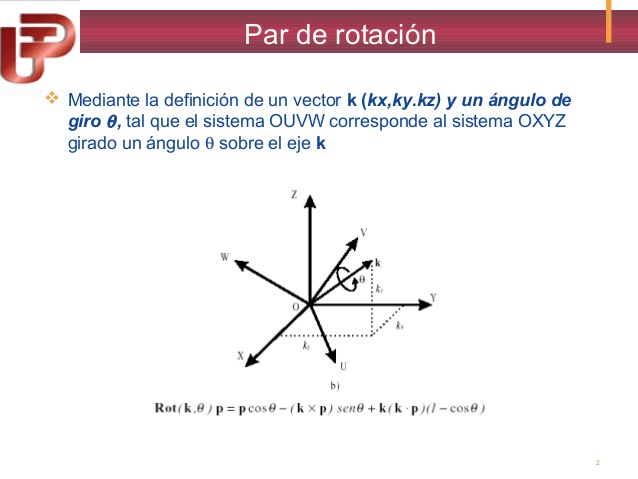
\includegraphics[width=0.8\textwidth]{robotica-cinematica2-2-638.jpg}\\ \\ \\ \\
Los cuaterniones unitarios proporcionan una notación matemática para representar las orientaciones y las rotaciones de objetos en tres dimensiones. Comparados con los ángulos de Euler, son más simples de componer y evitan el problema del bloqueo del cardán. Comparados con las matrices de rotación, son más eficientes y más estables numéricamente. Los cuarteniones son útiles en aplicaciones de gráficos por computadora, robótica, navegación y mecánica orbital de satélites.\\ \\
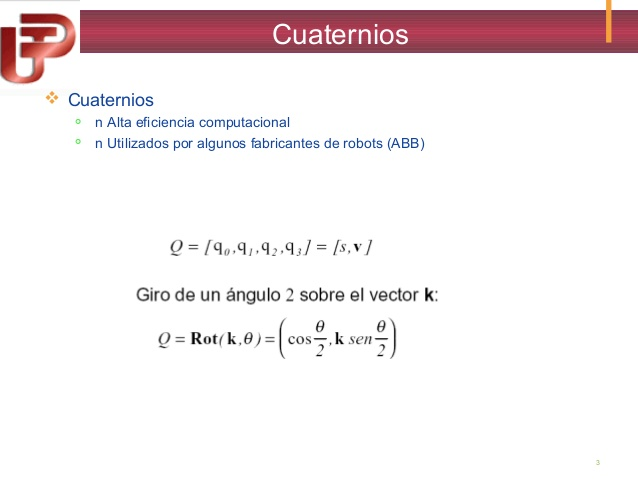
\includegraphics[width=0.7\textwidth]{cuaternio.jpg}
\vspace{5.5cm}

\bibliographystyle{plain}
\bibliography{biblio}



\end{document}